% Source: report/sections/05_speed.md (owner: Trivedh, #4).
\section{Accuracy vs inference speed}
\label{sec:speed}
A segmentation model is only useful at the bedside if it can keep up with live colonoscopy video, which
arrives at \textbf{25--30 frames per second}. This section measures whether our five models can, and what it
costs to make them more accurate.

\paragraph{Measurement protocol (\texttt{fps()} in \texttt{common.py}).}
\begin{itemize}
  \item \textbf{Batch size 1.} Live video arrives one frame at a time, not as a batch, so batching would overstate
        real-world throughput.
  \item \textbf{Input $352\times352$}, the same resolution every model trains and evaluates at, run on a Kaggle \textbf{T4} GPU.
  \item \textbf{20 warm-up calls, not timed.} The first calls to a GPU model are slow: CUDA allocates memory and cuDNN
        benchmarks several convolution algorithms before picking the fastest one. Timing these would measure
        one-off setup cost, not steady-state speed.
  \item \textbf{200 timed calls}, with \texttt{torch.cuda.synchronize()} immediately before and after the timed block. GPU
        calls are asynchronous (the Python call returns as soon as the work is \emph{queued}, not when it finishes),
        so without synchronising, the measured time would be wrong (usually far too short).
  \item Reported as \textbf{\texttt{fps\_fp32}}, \textbf{\texttt{fps\_fp16}} (mixed precision) and \textbf{\texttt{fps\_fp16\_tta}} (fp16 with test-time
        augmentation, see below). Mixed precision is not a uniform win: see ``Does fp16 always help?'' below; the
        gain depends on the architecture, and for one model (SegFormer) fp16 is actually slower.
  \item \textbf{ms per frame = 1000 / FPS}, the number that actually determines whether a frame is processed before
        the next one arrives.
\end{itemize}

\paragraph{Test-time augmentation (TTA).}
For each frame we predict on the original image and on its horizontal flip, vertical flip, and both flips
combined, flip each prediction back to the original orientation, and average the four. Averaging smooths
out orientation-dependent errors, so it usually improves Dice a little (\texttt{dice\_tta}). \texttt{fps()} times this as
\textbf{one batch of 4} (the four flipped views go through the model together), not as four separate forward
passes, so the throughput cost is not a fixed ${\sim}4\times$: it depends on how well each architecture's layers batch,
and ranges from $1.3\times$ to $3.2\times$ across our five models (see below). \Cref{fig:tta} plots this
trade-off for our two pretrained CNN U-Nets: an arrow from the no-TTA point to the TTA point of the same model,
right-to-left meaning slower and upward meaning more accurate.

\begin{figure}[t]
  \centering
  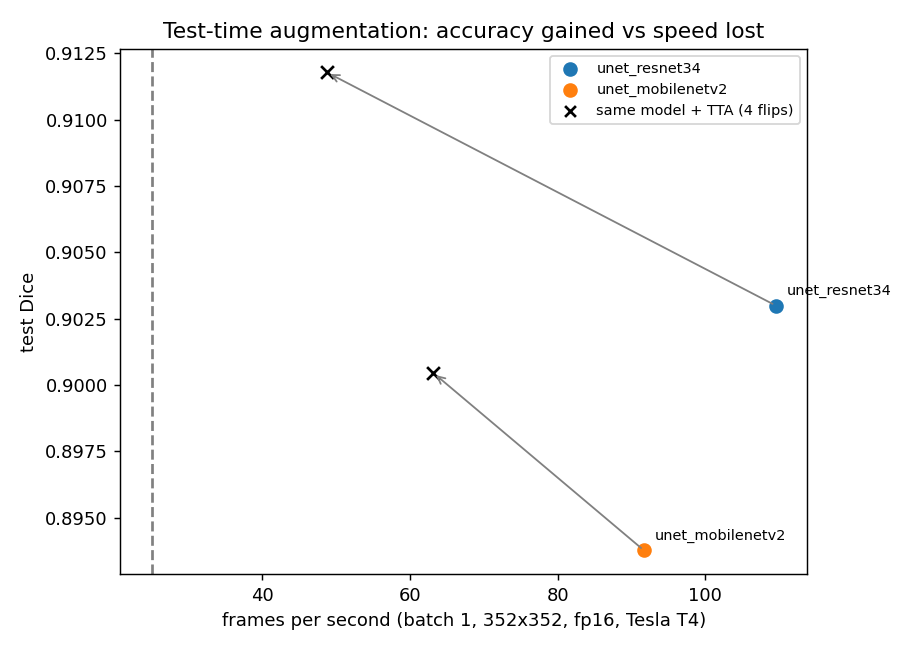
\includegraphics[width=\linewidth]{tta_tradeoff.png}
  \caption{Test-time augmentation for the two pretrained CNN U-Nets: each arrow goes from the model without TTA to the same model with TTA.}
  \label{fig:tta}
\end{figure}

\begin{table*}[t]
  \centering
  \small
  \begin{adjustbox}{max width=\textwidth}
  \begin{tabular}{@{}lccccccc@{}}
    \toprule
    Model & Params (M) & FPS fp32 & FPS fp16 & FPS fp16+TTA & ms/frame (fp16) & Dice & Dice+TTA \\
    \midrule
    U-Net (scratch)     & 31.0 & 11.6 & 45.7  & 14.7 & 21.9 & 0.851 & 0.863 \\
    U-Net + ResNet-34   & 24.4 & 44.9 & 109.5 & 48.7 & 9.1  & 0.903 & 0.912 \\
    U-Net + MobileNetV2 & 6.6  & 86.5 & 91.7  & 63.1 & 10.9 & 0.894 & 0.900 \\
    Attention U-Net     & 31.4 & 10.6 & 40.7  & 12.7 & 24.6 & 0.854 & 0.857 \\
    SegFormer (MiT-B2)  & 24.7 & 56.9 & 43.3  & 32.8 & 23.1 & 0.917 & 0.926 \\
    \bottomrule
  \end{tabular}
  \end{adjustbox}
  \caption{Inference speed (batch 1, $352\times352$, T4 GPU) and test Dice of all five models.}
  \label{tab:speed}
\end{table*}

\paragraph{Which models reach 25 FPS.}
\textbf{In fp16}, all five models clear 25 FPS without TTA (\cref{tab:speed}), from the slowest (Attention U-Net, 40.7 FPS) to the
fastest (ResNet-34, 109.5 FPS): at this resolution, fp16 throughput is not the bottleneck for any of them.
\textbf{In fp32}, the picture is different: the scratch U-Net (11.6 FPS) and Attention U-Net (10.6 FPS) fall well
short of 25 FPS, because they apply full $3\times3$ convolutions at full resolution and through a 1024-channel
bottleneck, far more computation per frame than the pretrained encoders, which downsample early. In fp16
the T4's tensor cores absorb most of that cost; only ResNet-34 (44.9), MobileNetV2 (86.5) and SegFormer
(56.9) clear 25 FPS in fp32 itself.

With TTA (always timed in fp16), the scratch baseline and Attention U-Net both drop below the real-time
threshold (14.7 and 12.7 FPS), while ResNet-34 (48.7), MobileNetV2 (63.1) and SegFormer (32.8) stay above
it. MobileNetV2 does \textbf{not} keep the largest margin in every configuration: in fp16 without TTA, ResNet-34
is faster (109.5 vs 91.7 FPS); MobileNetV2 leads only in fp32 (86.5) and in fp16+TTA (63.1), where its
depthwise-separable blocks batch the four TTA views more cheaply. This matters in practice because a
deployed system also spends time on video decoding, pre/post-processing and display, not just the model's
forward pass: the raw FPS number is a ceiling, not what the clinician actually gets.

\paragraph{Is TTA worth it?}
TTA buys a small Dice gain for every model (+0.003 to +0.012) at a cost in frames per second that varies a
lot by architecture: $3.1\times$ for the scratch baseline ($45.7 \rightarrow 14.7$), $3.2\times$ for Attention U-Net ($40.7 \rightarrow 12.7$),
$2.25\times$ for ResNet-34 ($109.5 \rightarrow 48.7$), $1.45\times$ for MobileNetV2 ($91.7 \rightarrow 63.1$) and $1.32\times$ for SegFormer
($43.3 \rightarrow 32.8$). The two models whose fp16 speed already sits close to the 25 FPS floor (the scratch baseline
and Attention U-Net) are pushed below it by TTA; the other three stay above it, with MobileNetV2 keeping the
most headroom (63.1 FPS) and SegFormer the least (32.8 FPS, still about 31\% above the floor).

\paragraph{Does fp16 always help?}
No, the gain is model-dependent. Going from fp32 to fp16 speeds up the standard-convolution U-Nets a lot
(scratch $3.9\times$, Attention U-Net $3.8\times$, ResNet-34 $2.4\times$), but MobileNetV2 gains only $1.06\times$ ($86.5 \rightarrow 91.7$): its
depthwise convolutions make little use of tensor cores, and at this size per-layer overhead dominates.
SegFormer is \textbf{slower} in fp16 than in fp32 ($56.9 \rightarrow 43.3$): mixed precision adds type casts, and its
attention and normalisation layers gain little from it. The practical conclusion is that each model should
be deployed in whichever precision is actually faster for it: fp16 for the four U-Net variants, but fp32
for SegFormer.

\paragraph{Recommendation.}
Across all five models, two poles stand out. SegFormer (MiT-B2) is the most accurate model we trained,
Dice 0.917 [95\% CI 0.893, 0.937], rising to 0.926 with TTA, and it still clears the real-time floor with TTA
at 32.8 FPS (about 31\% above 25 FPS), but it must be deployed in \textbf{fp32} (56.9 FPS without TTA) to reach
its best speed, not fp16. U-Net + MobileNetV2 trades some of that accuracy for raw speed headroom: Dice
0.894 [0.862, 0.921] (0.900 with TTA) but 63.1 FPS with TTA, at only 6.6\,M parameters.

A paired bootstrap over the same 120 test images (2000 resamples, the method of \cref{sec:ci}) shows SegFormer's
edge over MobileNetV2 is real (+0.023 Dice [0.008, 0.040], $p = 0.005$), and MobileNetV2 also has the highest
miss rate of the three fast models (5.0\% vs SegFormer's 2.5\%) and the largest accuracy drop of all five
models on the out-of-distribution CVC-ClinicDB set (0.141, more than the scratch baseline's 0.101), a
generalisation concern beyond raw Dice.

U-Net + ResNet-34 sits between the two poles: Dice 0.903 [0.874, 0.928] (0.912 with TTA), not significantly
different from either SegFormer (+0.014 [$-$0.006, 0.036], $p = 0.17$) or MobileNetV2 (+0.009 [$-$0.009, 0.027],
$p = 0.33$) on our 120 test images; with $n = 120$ the test has little power, so ``not significant'' is not the
same claim as ``the same''. By speed: ResNet-34 reaches 109.5 FPS in fp16 without TTA, about $1.9\times$ SegFormer's
best (56.9 FPS in fp32 without TTA), or 48.7 FPS in fp16 with TTA against SegFormer's 32.8 FPS in fp16 with
TTA (SegFormer with TTA was only measured in fp16, not fp32). ResNet-34 also generalises to CVC-ClinicDB far
better than MobileNetV2 (drop of 0.075 vs 0.141).

Our recommendation: \textbf{SegFormer, run in fp32 (56.9 FPS without TTA, 32.8 FPS in fp16 with TTA), where
accuracy is the priority}, and \textbf{U-Net + ResNet-34, run in fp16 (109.5 FPS without TTA, 48.7 FPS with
TTA), where real-time speed matters most}: its Dice is not significantly different from SegFormer's on
our 120 test images ($p = 0.17$) while it is markedly faster and more robust on CVC-ClinicDB than MobileNetV2.
We do not recommend MobileNetV2 for deployment despite its FPS headroom, given its weaker generalisation and
higher miss rate.
